In this chapter, we begin with presenting the necessary background to understand the CNNs for classification and feature extraction task, training data arrangement procedures, and instance selection methods, as well as other ideas required to understand our research. We start with the typical structure of CNNs and the gradient descent training method. We then discuss the advanced training set arrangement methods that can speed up the training procedure and outline their deficiencies for our purpose. Next, we review the instance selection literature and present a CNN instance selection pipeline - use the network pre-trained on ImageNet to extract low-dimensional features and run the instance selection methods on extracted features. Furthermore, we cover the existing trade-off framework BlinkML \cite{Park2019a} in the context of maximum-likelihood estimation machine learning algorithms and explain why it is not suitable for the deep neural network. Finally, we present TAPAS \cite{Istrate2019}, which is an accuracy predictor for the deep neural network without training and has several properties that make it useful to build our trade-off framework.


\section{Classification and Feature Extraction with CNNs}
\label{slcnn}
Classification is a kind of machine learning task which learns the mapping between visual inputs and output labels from a set of well-labelled training samples. The visual data can be images, videos or even 3D models \cite{Song2020}. The output scores after a softmax operation can be considered as the probability for a given image belonging to each class. We use the symbol $P(c|x, \theta)$ to represent the probability that sample $x$ belongs to true class $c$. The scores of true classes also reflect the difficulties for CNNs to classify the samples correctly. Higher scores indicate the samples are easier to classify than lower score samples. CNNs are particular tools that can solve this task. They are a set of chained operations with trainable parameters. These parameters define the actual input-out mapping. For this reason, we use the symbol $f(x|\theta)$ to represent the output score of true class predicted by the CNNs, which takes the input $x$ with a particular parameter set $\theta$. 

Figure \ref{Fig.CNN} gives a basic CNN structure which is optimised to classify images as cats or dogs. It contains two convolutional (Conv) layers, one max-pooling layer and one fully connected (FC) layer. The last FC layer is a multi-class logistic regression model which maps the outputs of the max-pooling layer to the classification scores. From this perspective, we can divide the CNN structure into two parts: feature extraction part and logistic regression part. The feature extraction part performs as a black box which ideally transforms the input images to points in a lower-dimensional, linearly separable space. 

 \begin{figure}[H]
 \centering
 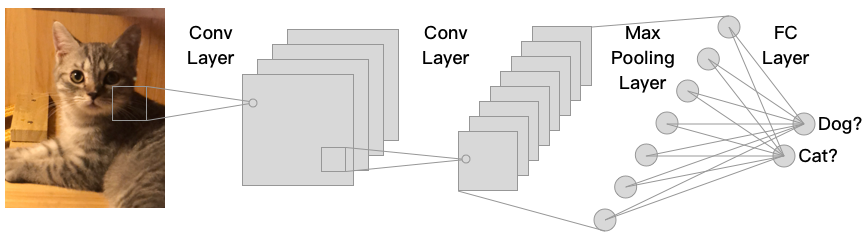
\includegraphics[width=0.8\textwidth]{src/CNN.png}
 \caption{A basic CNN structure to classify images between cats and dogs. The outputs of the penultimate FC layer are the extracted lower-dimensional features of the input images. These features should be linearly separable to achieve a high classification accuracy.}
 \label{Fig.CNN}
 \end{figure}



We use the symbol $y$ to represent the ground truth of the input sample $x$. The equation $L(f(x|\theta), y)$ represents the loss function which measures the difference between the predicted output and the ground truth label. Then the training process is to find the parameter set $\theta^*$, which minimise the average loss of the whole training set as follows:
\begin{equation}
\label{dlopt}
\theta^* = \mathop{\arg\min}_{\theta}\ \frac{1}{N}\sum^{N}_{i=1}L(f(x_i|\theta), y_i)
\end{equation}

where the symbol $N$ stands for the number of samples in the training set. This equation turns the training process into an optimisation problem. Different from machine learning algorithms like logistic regression and SVM, the equation \ref{dlopt} is non-convex thus cannot be solved analytically \cite[p.~304]{Courville2016}. Several techniques have been developed to solve this problem with the requirement that the loss function $L(.,.)$ is differentiable. The basic one is called stochastic gradient descent (SGD) which updates the parameters with the partial derivatives of a randomly selected sample. At each step, the new parameter is calculated with: 

\begin{equation}
	\theta_{t+1} = \theta_t - \eta
 \frac{\partial{L(f(x|\theta), y)}}{\partial{\theta_t}}
\end{equation}
and $\eta$ is the step size. A simple variant of SGD is mini-batch gradient descent which divides the training set into disjoint subsets and averages the gradients within the subset before updating the parameters:

\begin{equation}
	\theta_{t+1} = \theta_t - \eta \frac{1}{M} \sum_{i=1}^{M}
 \frac{\partial{L(f(x_i|\theta), y_i)}}{\partial{\theta_t}}
\end{equation}
where $M$ is the batch size of the subset. For CNNs, batch size $M$ is often smaller than the training set size $N$ because it takes too much memory to fit in the whole dataset. Usually, we use the value 128 or 256 as the batch size. 

The feature extraction method mentioned above is to train a network first then take the penultimate FC layer outputs. In practice, this is not efficient nor effective. If we have an extensive training set, it takes us too many resources to train them well \cite{Chen2016}. If we have a small training set, it may be hard to acquire high-quality features. An alternative method is to extract the features with a pre-trained network. Typically we use the weights trained on ImageNet \cite{Russakovsky2015} because this dataset is large enough and the pre-trained network can extract good enough features for other datasets \cite{Kornblith2018}.


\section{Training Set Arrangement}
Since the mini-batch gradient method trains the network with a subset of samples at each step, how to select the samples becomes a problem in the deep learning literature. Instead of uniform sampling, many researchers proposed to select the samples with sample weights based on different criteria. In this section, we plan to introduce the current hypothesis methods and target hypothesis methods. Current hypothesis methods measure the samples based on the parameter set $\theta_t$ at step $t$ while target hypothesis methods are based on the final optimal parameter set $\theta^*$. 

\subsection{Current Hypothesis Methods}
Different authors have proposed a variety of current hypothesis methods. Specifically, in self-paced learning \cite{Kumar2010, Li2017, Meng2016}, active bias learning \cite{Chang2017}, and hard example mining \cite{Shrivastava2016, Loshchilov2015}, the batch selection process is based on the classification scores $f(x|\theta, y)$. For importance sampling methods, the process is based on the gradient norm for each sample, $|\frac{\partial{L(f(x_i|\theta), y_i)}}{\partial{x_i}}|$. We finish this section by briefly explaining the theories of these approaches.

\subsubsection{Difficulty Based Methods}

Self-paced learning tends to select easy samples which have a high classification score by injecting a pace function into the optimisation target function \ref{dlopt}:
\begin{equation}
\label{spl}
\theta^* = \mathop{\arg\min}_{\theta, v}\ \sum^{N}_{i=1} v_iL(f(x_i|\theta), y_i) + \lambda \sum^{N}_{i=1}  v_i
\end{equation}
where $v$ is the sample weight calculated by the pace function. The pace function can be either a simple step function \cite{Kumar2010} or a more complicated dynamic function which changes while training $t$ \cite{Li2017} as long as it can assign weight 0 to samples. By minimising the target function \ref{spl}, this method would zero out hard examples which have higher loss values, thus keeps only the easy samples. With self-paced learning, the trained network can be more robust to outliers \cite{Meng2016}.

A potential problem of self-paced learning is that it would gradually increase the loss of hard examples \cite{Kumar2010}. As a consequence, the trained network may not achieve the desired accuracy. The possible solution is to use the active bias learning method, which is designed to select the uncertain samples whose classification scores fluctuate near the decision threshold. Chang et al. proposed and evaluated many self-paced methods, and the representative one is  SGD Sampled by Threshold Closeness (SGD-STC) \cite{Chang2017}. It records the historical average classification probability $\bar{P}$ for each sample. The sample weights are calculated with an equation that is proportional to $(1-\bar{P}) \times \bar{P}$ whose maximum point is at $\bar{P} = 0.5$. However, the problem is that we need extra space and computation to maintain historical scores.

Hard example mining is yet another heuristic method aims at maximising the convergence speed by extending the self-paced learning method \cite{Shrivastava2016}. The algorithm proposed by \cite{Loshchilov2015} ranks the samples based on the latest computed classification score in descending order. At early training stages, the algorithm chooses easy samples just like self-paced learning. After a thorough training process, the algorithm tends to select hard examples which have low classification scores. In this way, the trained classifier may be able to achieve higher accuracy than self-paced learning. The downside is that training with hard examples can affect the decision boundary. As a consequence, the network may forget learned features previously and reduce the accuracy. 



\subsubsection{Importance Based Methods}
\label{ibalgorithm}
Although experiments in the cited resources above have proved that difficulty based methods can surely speed up the training process and may achieve even higher accuracy, the lack of mathematical prove could lower the interests of researchers. On the contrary, importance based methods raise from the profound mathematical demonstration \cite{Zhao2015} and are more reliable. Despite the elaborate derivation, the most important conclusion is that the optimal weight distribution is proportional to the per-sample gradient norm.

The challenge is that computing the per sample gradient norm $|\frac{\partial{L(f(x_i|\theta), y_i)}}{\partial{x_i}}|$ is intractable. In the past few years, many researchers have adapted their approximate methods to speed up the process. The most convincing one is proposed by Katharopoulos et al. which derives an upper bound of the gradient norm \cite{Katharopoulos2018},

\begin{equation}
	|\frac{\partial{L(f(x_i|\theta), y_i)}}{\partial{x_i}}|  \leq |h(x_i)|\end{equation}
that $h(x_i)$ is the upper bound function depends on the last layer pre-activation outputs. With this equation, we can compute the largest sample gradient after a single forward propagation. 

The benefit of current hypothesis methods is that the sample weights vary with training step. Thus the chosen samples at each step can reflect the current capacity of the network. However, because evaluating the whole training set is time-consuming, we often select a subset uniformly first and then select the samples within the subset. As a result, we can only get a sub-optimal choice which is no better than the theory performance. 

\subsection{Target Hypothesis Methods}
Compared with the current hypothesis methods, target hypothesis methods arrange the training set based on the possible final classification scores of the network thus the weights of the samples are pre-defined. They will not change during the training process \cite{Bengio2009}. For this reason, the target hypothesis method is more suitable to reduce the size of the datasets. To our knowledge, Curriculum Learning (CL) is the only method with these properties, as stated by Hacohen et al. in 2019 \cite{Hacohen2019a}.

Similar to hard example mining, CL trains the network with easy samples first. Rather than switching to difficult samples, CL adds difficult samples into the training set. Eventually, the subset would contain all the training samples. The classification scores are measured with a pre-trained network or with a linear classifier such as SVM \cite{Hacohen2019a}. The major concern is that CL weights may not reflect the sample classification difficulties of the chosen CNN. Considering the reality that all methods described above are sub-optimal in practice, we choose to accept the drawbacks in this project.

The Python style \footnote{We use Python objects and their functions such as .append().} pseudo-code of CL is shown in Algorithm \ref{CL-implement}. In this dissertation, we assume the type of input feature vector is NumPy array.  

% CL

\begin{algorithm}[H]
\label{CL-implement}
 \KwData{image feature vectors $M$}
 \KwIn{number of samples to select $m$, classification score for each sample $scores$, number of classes $n$}
 \KwOut{selected sample index by CL}

$selected\_idx\_list = []$ \footnote{All variables ended with the postfix \textit{\_list} are Python list objects.}\;

\ForEach{class label L}{
	scores = all sample scores with label L \;
	idx\_list = sort\_by\_value(scores) \;
	selected\_idx\_list.append(idx\_list[: floor(m/n)]) \;
}


\Return $selected\_idx\_list$ \;

\caption{CL}
\end{algorithm}

\section{Instance Selection Algorithm}
Most instance selection methods are designed to reduce the size of the structured dataset for machine learning algorithms like SVM and logistic regression. The assumption is that we can recover the decision boundary with fewer samples. According to the thorough review \cite{Olvera-Lopez2010}, the instance selection methods can be divided into two categories: wrapper and filter. Wrapper methods select the subset samples based on the classification results. K-NN \cite{Aha1991} is a common choice to evaluate classification quality. Misclassified samples will be selected because they can contribute to the K-NN accuracy. Filter methods select samples without repetitive evaluation. They tend to select samples near the boundary between different classes with the assumption that these samples can guide the classifiers to recover the position of the original decision boundary \cite{Riquelme2003a, Malhat2020}.  Although the wrapper methods could achieve higher accuracy because they are classifier dependent, they tend to cost too much time because they need to evaluate the accuracy multiple times. From this perspective, filter methods are more suitable for our experiments. In this section, we take two typical filter algorithms, POP and EGDIS, to introduce their mechanisms.

\subsection{Patterns by Ordered Projections}

% POP
The POP algorithm \cite{Riquelme2003a} is designed to select boundary samples by removing inner samples which are far from the class contour. Rather than calculating the sample positions in the high dimensional feature space, Riquelme et al. simplified this process by projecting the samples onto each feature dimension. To be precise, we decide if a sample is inner or not in each feature space. We use the term \textbf{pure inner samples} to refer to samples which are inner in all feature spaces. 

Algorithm \ref{pop_psudo} describes the POP pseudo-code. we use the variable $weakness$ to count the number of times that a sample is inner. In each feature dimension, the function $sort\_by\_value$ first sort the samples in descending order. Since our extracted features are continuous values, we need an extra hyper-parameter $equal\ tolerance (et)$ to decide when two feature values are equal. Then the function $resort\_by\_label$ scans the samples and record the start label of consecutive samples with the same value and detects the label of the first sample with a different value. Then the function sorts the scanned samples by moving samples with the same labels as the two recorded to the start of the list and the end of the list. After that, we scan all samples one more time to detect label changes and mark all samples as inner except the two at the beginning and the end of the scanned list. Figure \ref{Fig.pop_work_flow} depicts a typical work flow of the function $resort\_by\_label$.


 \begin{figure}[H]
 \centering
 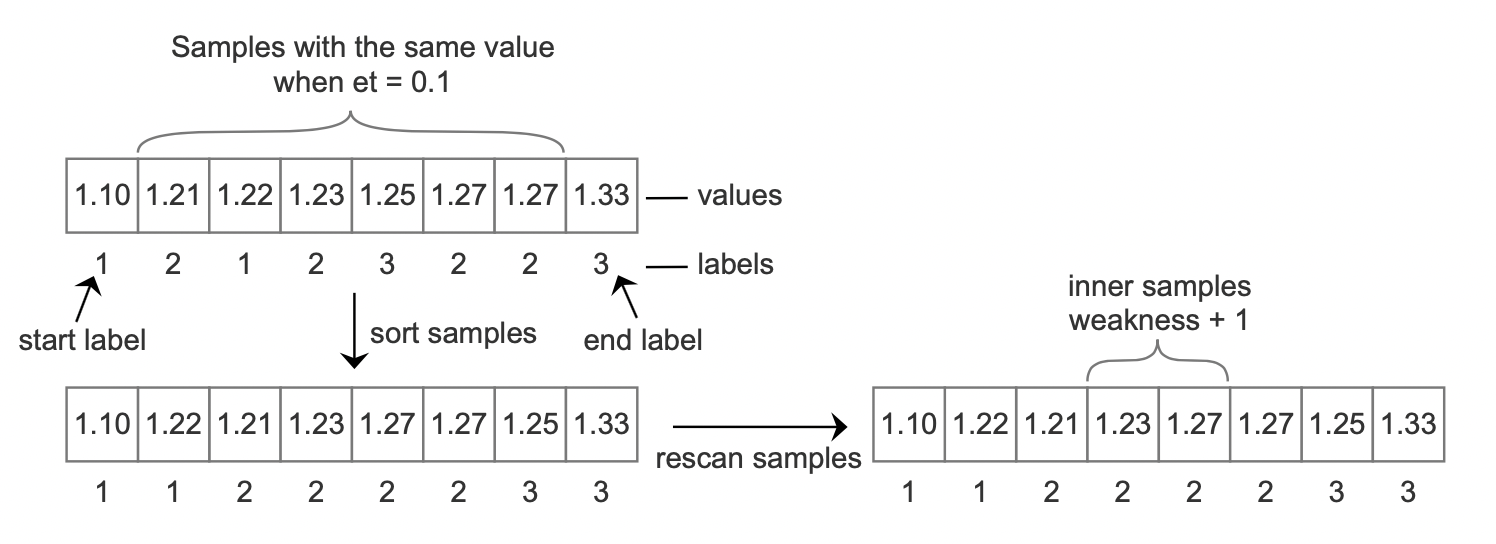
\includegraphics[width=1\textwidth]{src/pop_work_flow.png}
 \caption{The typical workflow of POP.}
 \label{Fig.pop_work_flow}
 \end{figure}


\begin{algorithm}[H]
\label{pop_psudo}
 \KwData{feature vectors $M$}
 \KwIn{weakness threshold $wt$, equal tolerance $et$}
 \KwOut{selected sample index by POP}
 

$weakness = np.zeros(len(M))$ \;

\ForEach{feature dimension $F_j = M[:,\ j]$} {
	 $idx\_list = sort\_by\_value(F_j)$ \;
	 $idx\_list = resort\_by\_label(F_j,\ et,\ idx\_list)$ \;
	 
	 \ForEach{idx in idx\_list} {
	 	\If{M[idx, j] is inner}{
	 		$weakness[idx] += 1$\;
	 	}
	 }
}

\Return $np.argwhere(weakness < wt)$ \;

\caption{POP for continuous features}
\end{algorithm}



% EGDIS

\subsection{Enhanced Global Density Based Instance Selection}
Similar to POP, EGDIS \cite{Malhat2020} aims at selecting boundary samples as well. Instead of removing inner samples,
EGDIS selects the boundary samples, which are close to other classes. It also selects samples at the densest area to capture some inner samples. The pseudo-code is shown in Algorithm \ref{EGDIS_code}. In order to find these samples, the function $kneighbours$ calculates the distances between the k neighbours. Then for each sample, we check how many neighbours are from other classes and save the value to variable $irrelevance score$. If the score is greater or equal to the integer part of $k/2$, we record this sample to the $boundary\_idx$ list. If not, function $density$ calculates the global density values:


\begin{equation}
	density(x_i) = -\frac{1}{N}\sum_{j\neq i}{distance(x_i, x_j)}
\end{equation} 

for the sample and its k neighbours. We add the sample to the $densest\_idx$ list if its density value is the highest compared with its k neighbours. According to the original paper, EGDIS performs better with global density function in terms of reduction rate \footnote{Reduction rate is the percentage of samples selected}. However, the compute time increases with the number of samples. We will explore possible solutions in Chapter 3.
 

\begin{algorithm}[H]
\label{EGDIS_code}
 \KwData{feature vectors $M$}
 \KwIn{number of neighbourhoods $k$}
 \KwOut{selected sample index by EGDIS}

$boundary\_idx = []$ \;
$densest\_idx = []$ \;
$neighbour\_distance\_list, neighbour\_index\_list = kneighbours(M, k)$ \;
\For{i in range(len(neighbour\_index\_list))} {
 	neighbour\_index = neighbour\_index\_list[i, :] \;
	irrelevance\_score = irrelevance(neighbour\_index) \;
	\eIf{irrelevance\_score is greater or equal to floor(k/2)} {
		boundary\_idx.append(k) \;
	}{\If{density(M[i]) is larger than density(M[neighbour\_index])} 
	{densest\_idx.append(i)}}
}

\Return $np.union1d(boundary\_idx, densest\_idx)$ \;

\caption{EGDIS}
\end{algorithm}

\section{Trade-off Framework}
The main drawback of the instance selection algorithms is that we cannot control how much data to select nor the minimum accuracy \footnote{Here we assume that reduce the number of samples would affect the classification accuracy, which is true from our CNN experiments.} that we can accept. Although there is one trade-off framework published by Park et al. \cite{Park2019a}, it can only work with for machine learning algorithms which can be optimised by the maximum likelihood method. Therefore, to work with CNNs, we need to build a new trade-off framework. 

In order to build the framework, the primary challenge is to find the relationship between required relative accuracy and the number of training samples needed. However, this is not straightforward because the optimisation of CNNs for classification tasks can be considered as a non-convex problem in most cases \cite[p.~114]{Goodfellow2016}. It is hard to get the final accuracy without a long time training. Some second-order method could find the zero gradient point, such as Newton’s method \cite{Xu2020}. However, they are still prone to local minimum points and not scale well to large CNNs \cite[p.~310]{Goodfellow2016}. For the reasons mentioned above, we tend to investigate experimental methods rather than analytical methods. 

In 2019, Istrate et al. published a paper aiming at predicting the accuracy without training the networks \cite{Istrate2019}. They built a Lifelong Database of Experiments (LDE) which stores a massive amount of training experiments on many CNN structures and datasets. When a new dataset is given, the framework TAPAS first train the data with a small probe CNN \cite{Scheidegger2018} for five epochs. The accuracy is recorded as the Dataset Characterisation Number (DCN). TAPAS then fetches experiments with similar DCN from the LDE. With these history data, a regression model is trained, which takes the network structure and DCN as inputs to predict the classification accuracies. Although it is not realistic for us to collect enough data for such a framework, TAPAS provides a working example that it is possible to build the trade-off framework based on experiment histories.